\section{Progress}
\label{sec:Progress}


\begin{figure}[t!]
\centering
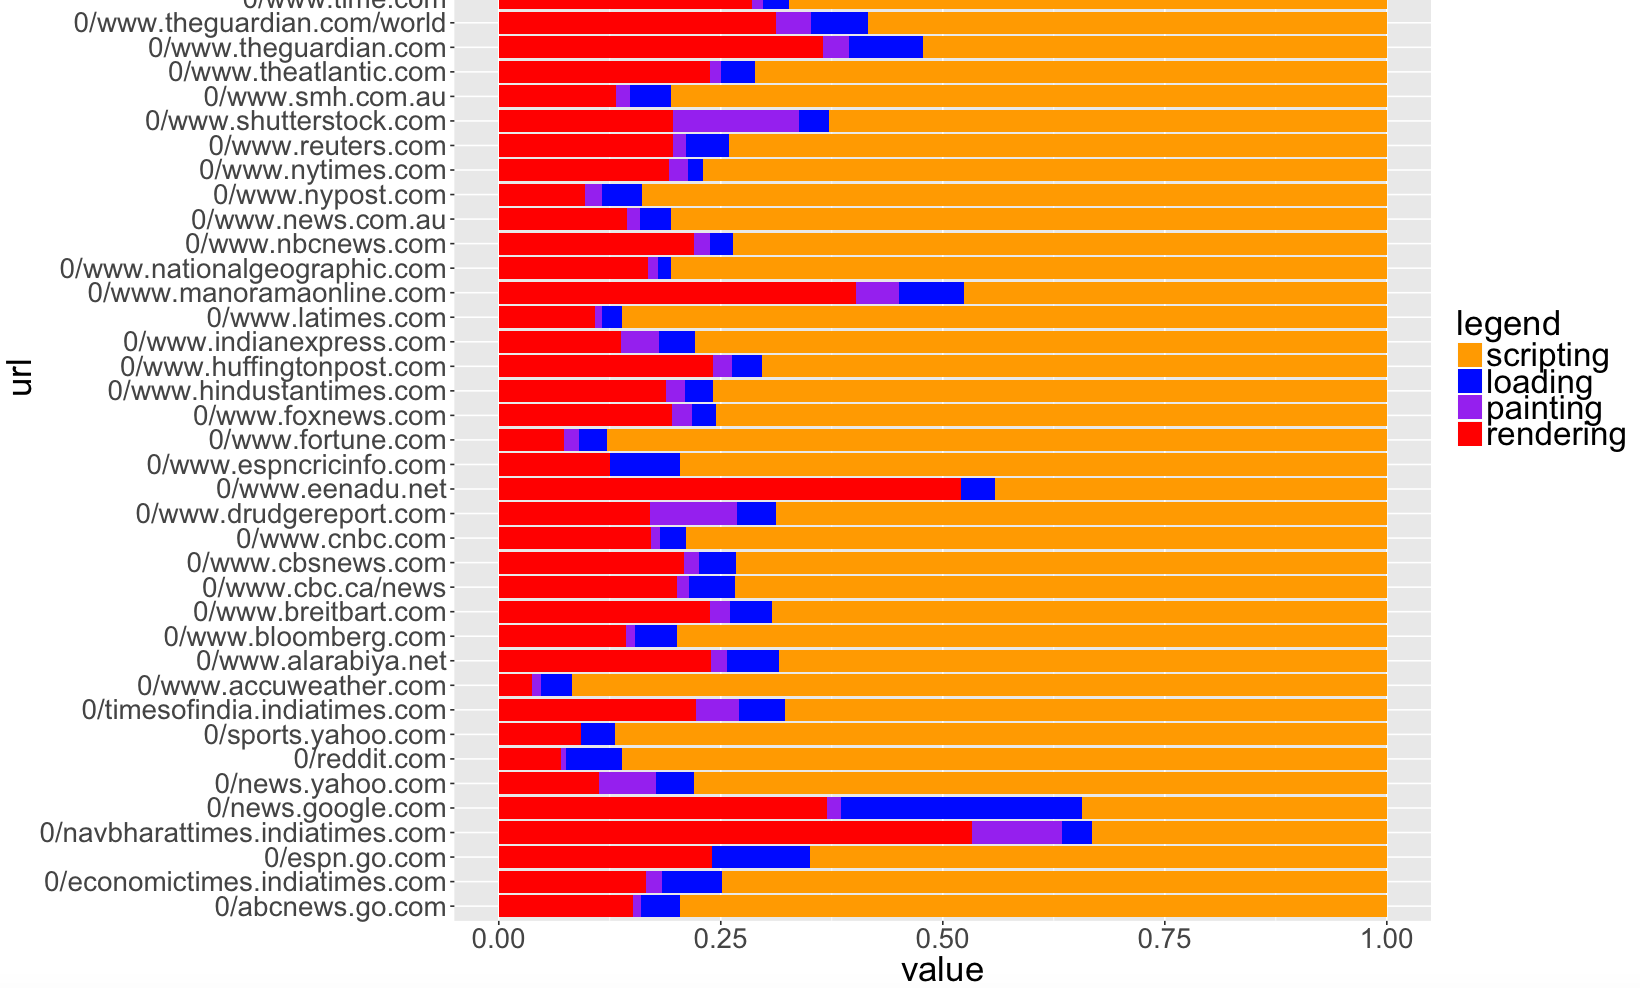
\includegraphics[width=0.99\columnwidth, scale=2.0]{figs/comp_1.png}
\tightcaption{Breakdown of computation on pixel 2}
\label{fig:act_p2}
\end{figure}

As a preliminary step, we first established a corpus of the top
75 news and sports websites to cater to the most popular and compute intensive websites. 
These websites were gathered from the Alexa top website list.
We ran all our experiments on a Google Pixel 2 with Chrome version 61. We leveraged chrome developer tools in order
to capture runtime traces for both networking and computation. We then analyzed these runtime
traces to draw insight into the critical path of the website, the total computation time vs the total networking time, and most importantly the finer
level breakdown of the computation time to understand the bottleneck of computation on mobile
devices. 

We categorized computation time into four categories: scripting, loading, rendering and
painting. Scripting is the total time spent on
compiling, evaluating and executing javascript. Loading consists of parsing the HTML and CSS, which happens 
immediately after the payload for the network requests are received by the browser. Loading
takes these payload objects and parses them before converting them to a DOM tree. Once the DOM tree is built,
the rendering engine converts this DOM tree into a render tree, which contains the
exact coordinates and the shape of each of the DOM nodes. This process comprises the rendering time of the web page.
Painting time is the time taken to process the render tree and convert
each pixel into a bitmap.
Figure 6 shows the computation breakdown for these four categories
on the Google Pixel 2. We further break down this time into the finer level events
which are returned by Google Chrome's trace and then group them by their event name.

\begin{figure}[t!]
\centering
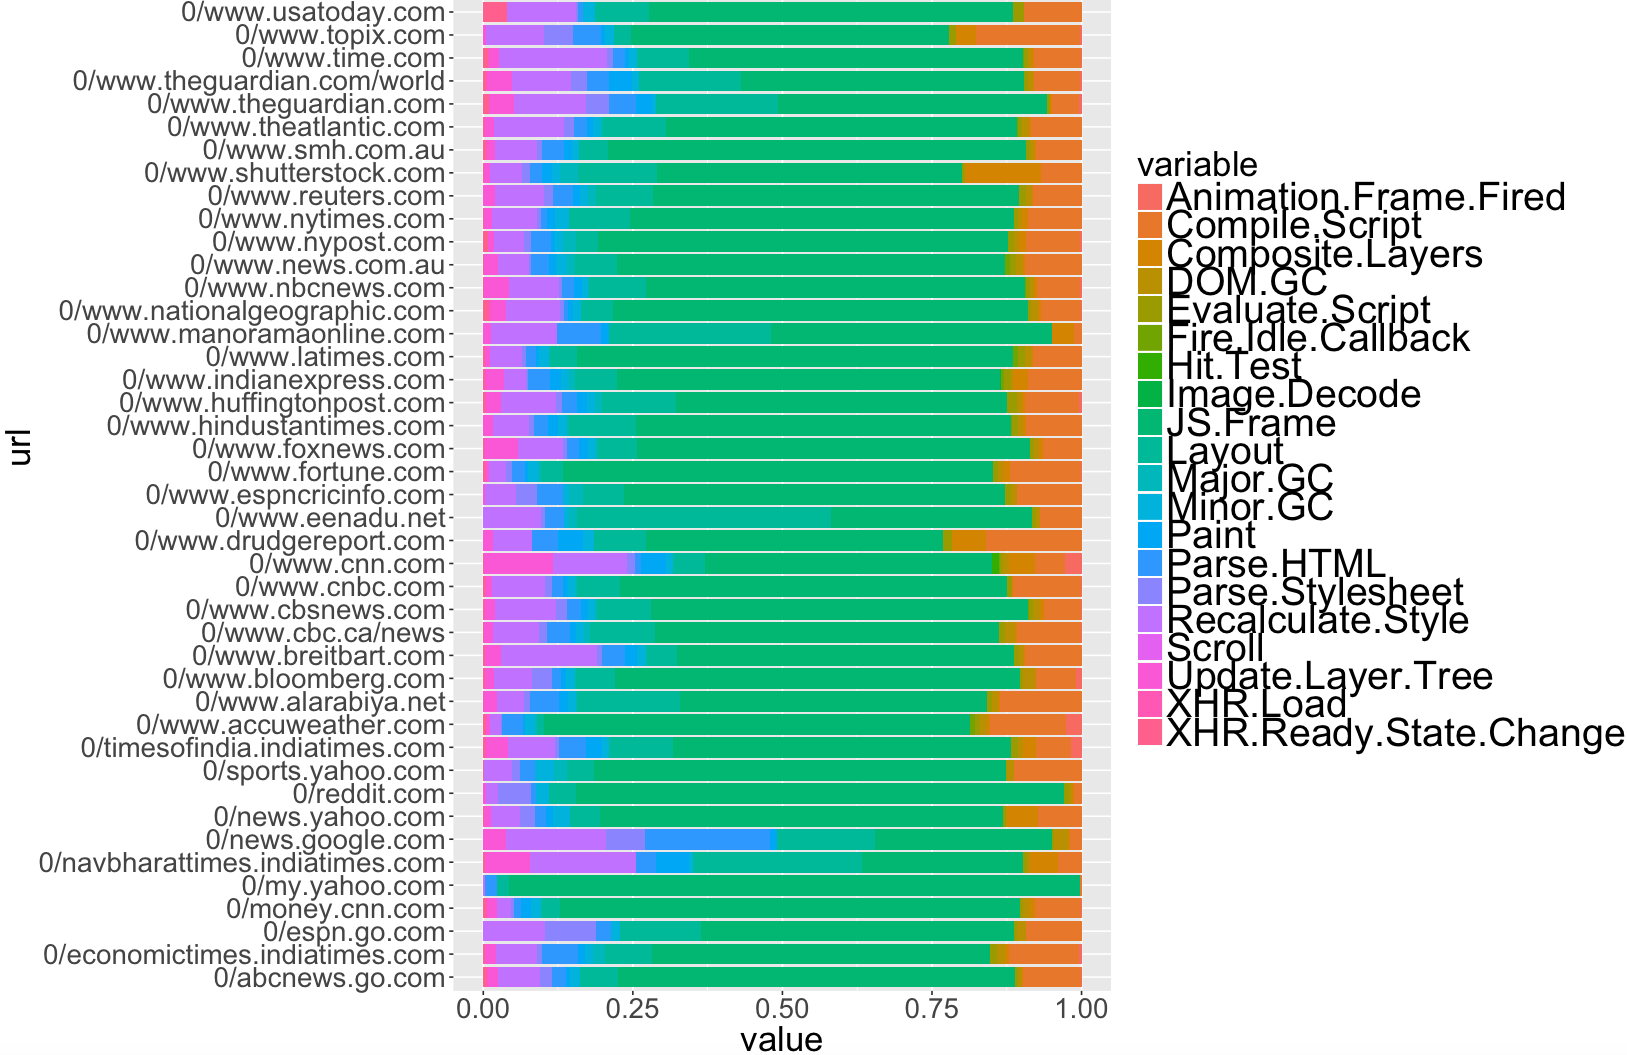
\includegraphics[width=0.9\columnwidth]{figs/comp_2.png}
\tightcaption{Breakdown of computation into finer events on pixel 2}
\label{fig:cat_p2}
\end{figure}


The results in Figure 7 show the promising impact a Javascript 
caching mechanism would have on the total page load time.

\subsection{Current Chrome Optimizations}

\begin{figure}[t]
\centering
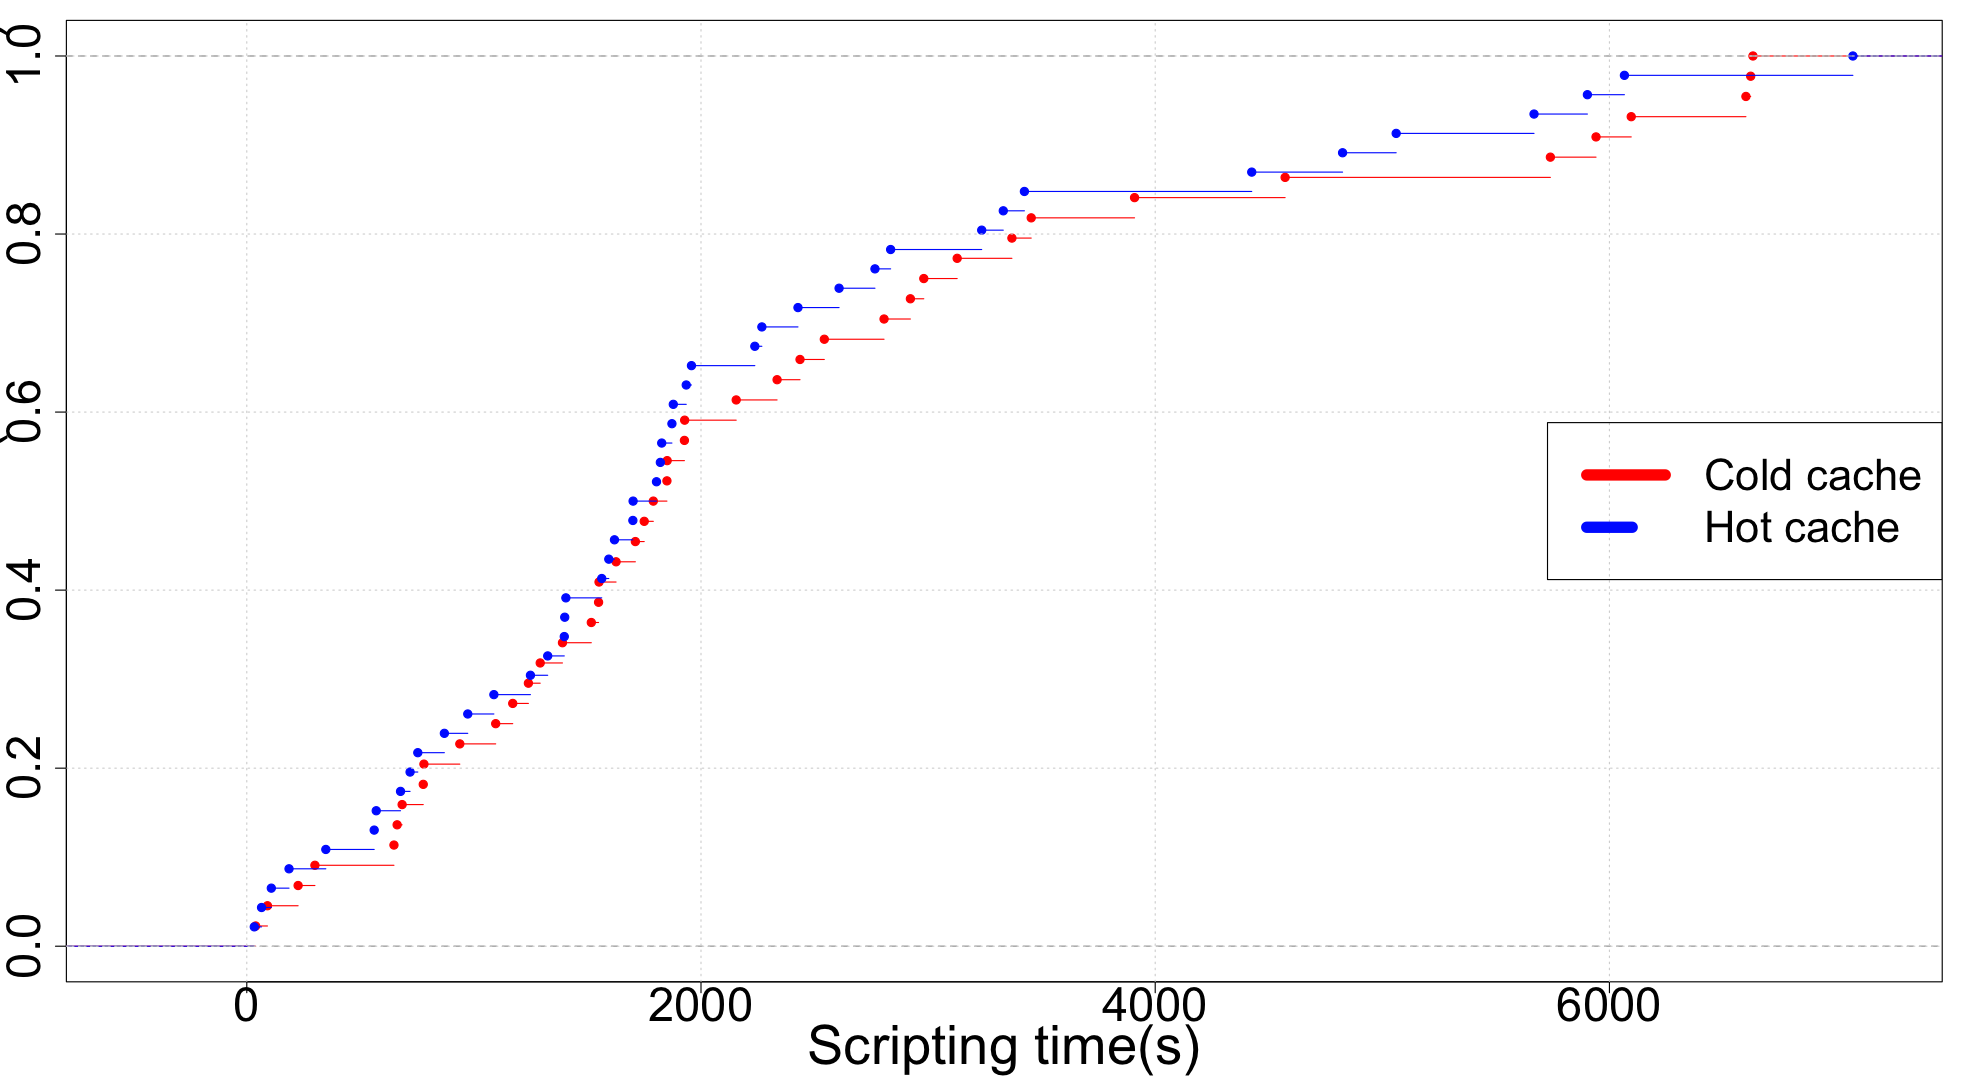
\includegraphics[width=0.9\columnwidth]{figs/chrome_script.png}
\tightcaption{CDF of scripting time with and without chrome's optimizations}
\label{fig:scripting_p2}
\end{figure}

Recently in their 2017 dev summit, the Chrome team discussed the various optimization techniques
they have developed to improve the total page load time.
We did a comparison of the total page load time with and without Chrome's optimizations to study
these improvements. We captured the trace from Alexa's top 75 
news and sports website once with a fresh cache, i.e. cold cache, and then subsequently with a hot
cache which contains all of Chrome's optimizations, including its compiler and parser cache. 
As seen in Figure 10, there has been a significant reduction in the overall compilation
time, with about 100ms reduction in median compile time. This is primarily due to the introduction of the compiler and parser cache. 
The line corresponding to cold cache refers to the fresh load of all the websites,
whereas the line corresponding to the hot cache refers to the subsequent load
which makes use of Chrome's caching framework. 
This is also reflected partially in the overall scripting time
as shown in Figure 8. Note that scripting time is the sum of compilation, execution and other
minor javascript events in the execution pipeline such as garbage collection. 
However, the interesting thing to note is that despite all these optimizations,
we observe almost negligible improvement in the median execution time of the Javascript, as
shown in Figure 9. This serves as motivation for the vast potential a caching framework would have in
improving the overall page load time.

\begin{figure}[t]
\centering
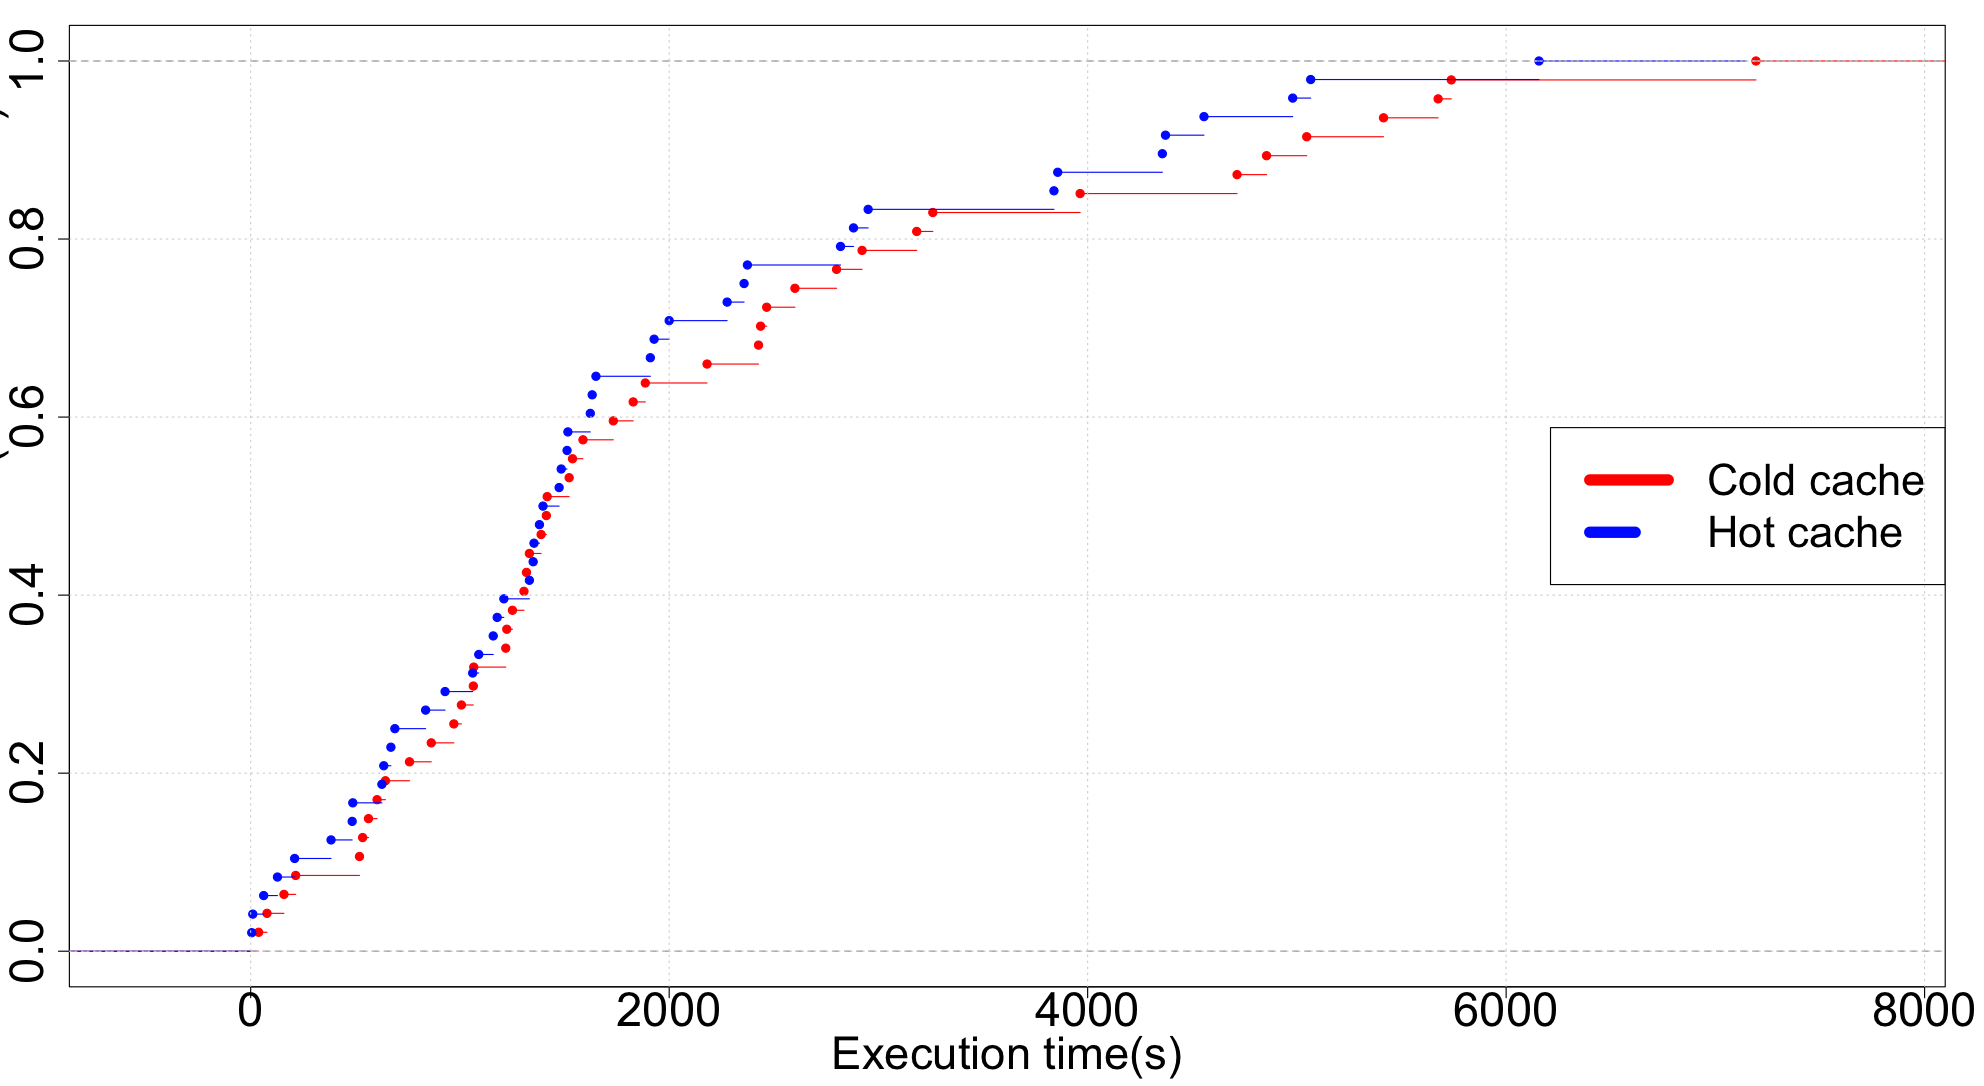
\includegraphics[width=0.9\columnwidth]{figs/chrome_exec.png}
\tightcaption{CDF of total execution time with and without chrome's optimizations}
\label{fig:compile_p2}
\end{figure}

\begin{figure}[t]
\centering
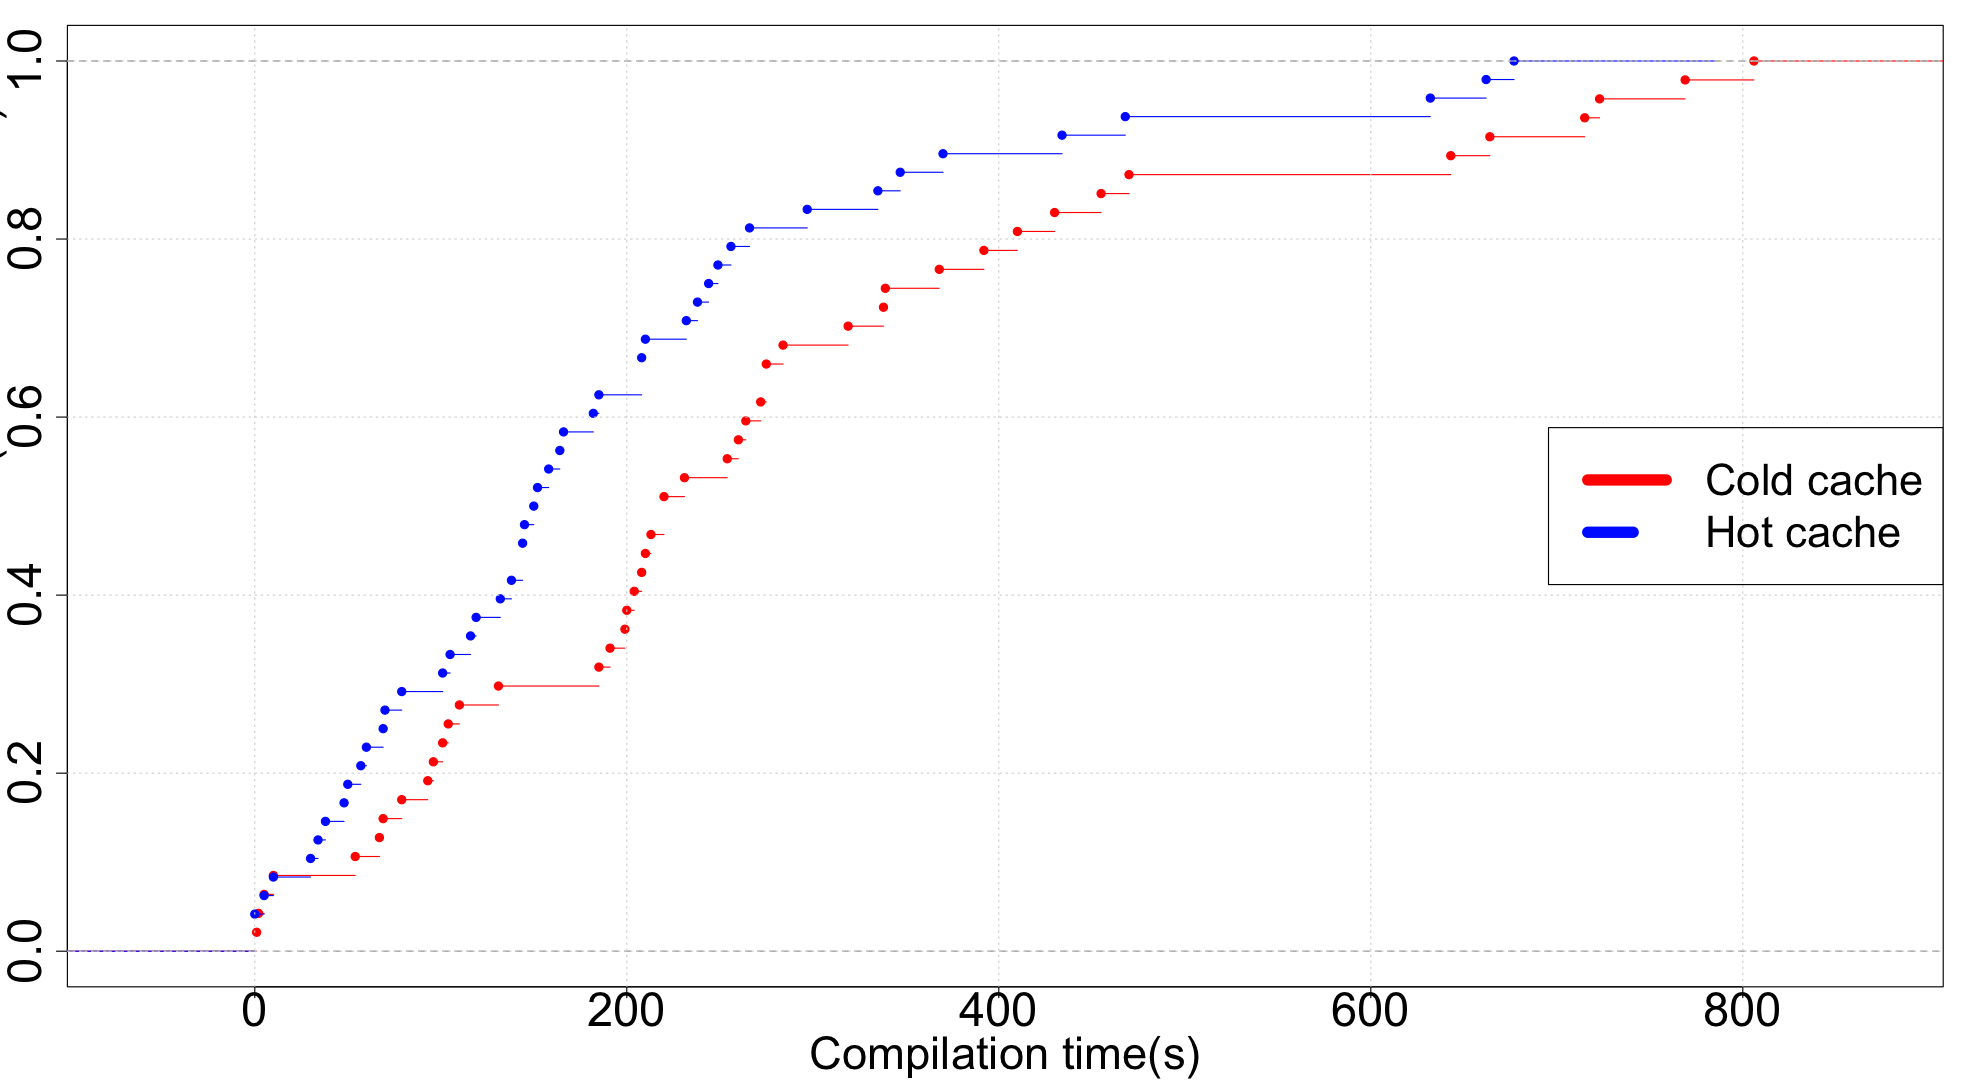
\includegraphics[width=0.9\columnwidth]{figs/chrome_compile.png}
\tightcaption{CDF of compilation time with and without chrome's optimizations}
\label{fig:compile_p2}
\end{figure}

\subsection{Experiments Conducted}

After establishing the impact of a Javascript execution caching framework, we conducted
experiments to understand Javascript computation at a finer granularity. We have explained the
results from these experiments in section 3.1. 
We observed that most of the properties of the global window object remain unchanged.
For a time difference of three seconds, we observe that only 2.5\% of properties
changed as shown in Figure 3. This is to be expected since little will change within three seconds 
of two subsequent web page loads. Surprisingly, even for a gap of three hours between
two loads, only 3.5\% of the properties changed as shown in Figure 4 and for a gap
 of three days, only 4.5\% 
properties changed. These are the 95\% percentile numbers, and therefore 
further motivate us to expect extremely high gains from a Javascript caching
framework. 

\begin{figure}[t]
\centering
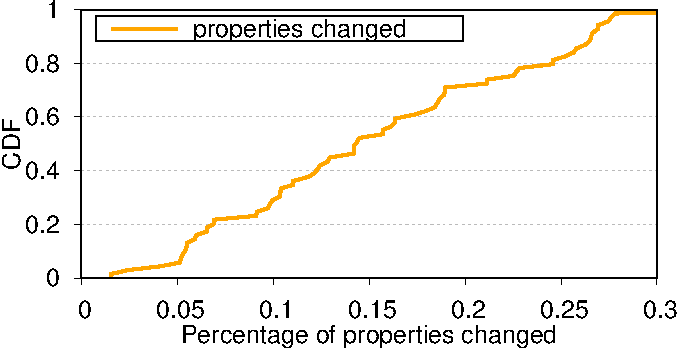
\includegraphics[width=0.9\columnwidth]{figs/cdf_bigdata_sec_new.pdf}
\tightcaption{Percentage of changed properties over 3 seconds}
\label{fig:properties-sec}
\end{figure}

\begin{figure}[t]
\centering
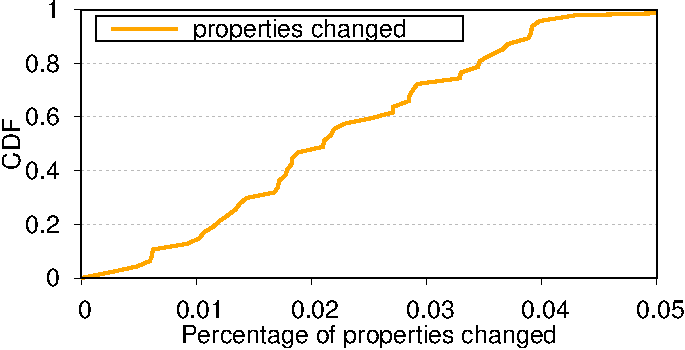
\includegraphics[width=0.9\columnwidth]{figs/cdf_bigdata_hr_new.pdf}
\tightcaption{Percentage of changed properties over 3 hours}
\label{fig:properties-hrs}
\end{figure}

\begin{figure}[t]
\centering
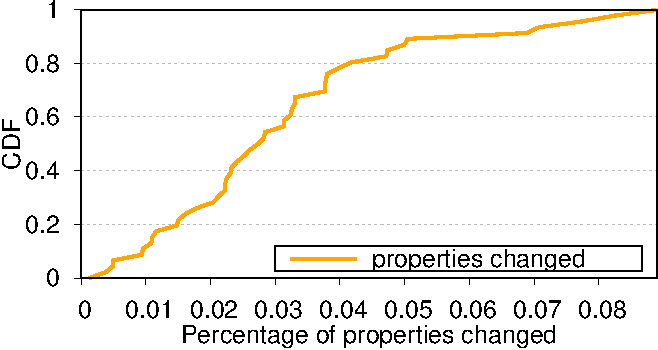
\includegraphics[width=0.9\columnwidth]{figs/cdf_bigdata_day_new.pdf}
\tightcaption{Percentage of changed properties over 3 days}
\label{fig:properties-day}
\end{figure}


Currently, we are working on capturing the Javascript execution at the function level. 
In order to do this, we have built
a web proxy which sits between the client browser and the news and sports websites. Every time 
a request is made by the client, the proxy intercepts the request, injects instrumentation
code in the javascript files, and injects inline script tags inside the HTML files. 
This instrumented code is read by the Javascript debugger when the page is loaded, and 
the debugger then builds a call graph, with each node representing a function that was invoked. 
Once a graph is built, we will use a graph diffing algorithm to quantify
how much of the call graph was modified across the two loads. 

